% -*- TeX -*-
\documentclass[aspectratio=169]{beamer}

\title{PyLith v4.1 Tutorial}
\subtitle{Quasistatic Elasticity with Time-Dependent Prescribed Fault Slip}
\author{Brad Aagaard\\
  Charles Williams \\
  Matthew Knepley}
\institute{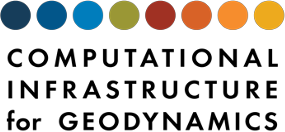
\includegraphics[scale=1.5]{../../logos/cig_logo_dots}%
  \hspace{4em}%
\raisebox{1em}{\includegraphics[scale=1.0]{../../logos/cig_short_pylith}}}
\date{June 11, 2024}


% ---------------------------------------------------- CUSTOMIZATION
\usetheme{CIG}
% Style information for PyLith presentations.

% Colors
\definecolor{ltorange}{rgb}{1.0, 0.74, 0.41} % 255/188/105
\definecolor{orange}{rgb}{0.96, 0.50, 0.0} % 246/127/0

\definecolor{ltred}{rgb}{1.0, 0.25, 0.25} % 255/64/64
\definecolor{red}{rgb}{0.79, 0.00, 0.01} % 201/0/3

\definecolor{ltpurple}{rgb}{0.81, 0.57, 1.00} % 206/145/255
\definecolor{purple}{rgb}{0.38, 0.00, 0.68} % 97/1/175

\definecolor{ltblue}{rgb}{0.2, 0.73, 1.0} % 51/187/255
\definecolor{mdblue}{rgb}{0.28, 0.50, 0.80} % 72/128/205
\definecolor{blue}{rgb}{0.12, 0.43, 0.59} % 30/110/150

\definecolor{ltltgreen}{rgb}{0.7, 1.00, 0.7} % 96/204/14
\definecolor{ltgreen}{rgb}{0.37, 0.80, 0.05} % 96/204/14
\definecolor{green}{rgb}{0.23, 0.49, 0.03} % 59/125/8
  
\definecolor{dkslate}{rgb}{0.18, 0.21, 0.28} % 47/53/72
\definecolor{mdslate}{rgb}{0.45, 0.50, 0.68} % 114/127/173
\definecolor{ltslate}{rgb}{0.85, 0.88, 0.95} % 216/225/229


\newcommand{\includefigure}[2][]{{\centering\includegraphics[#1]{#2}\par}}
\newcommand{\highlight}[1]{{\bf\usebeamercolor[fg]{structure}#1}}
\newcommand{\important}[1]{{\color{red}#1}}
\newcommand{\issue}[2]{\item[Issue:] {\color{red}#1}\\{\item[Soln:] \color{blue}#2}\\[4pt]}

\setbeamercolor{alerted text}{fg=ltgreen}
\setbeamertemplate{description item}[align left]


\newcommand{\lhs}[1]{{\color{blue}#1}}
\newcommand{\rhs}[1]{{\color{red}#1}}
\newcommand{\annotateL}[2]{%
  {\color{blue}\underbrace{\color{blue}#1}_{\color{blue}\mathclap{#2}}}}
\newcommand{\annotateR}[2]{%
  {\color{red}\underbrace{\color{red}#1}_{\color{red}\mathclap{#2}}}}
\newcommand{\eqnannotate}[2]{%
  {\color{blue}%
  \underbrace{\color{black}#1}_{\color{blue}\mathclap{#2}}}}

\newcommand{\trialvec}[1][]{{\vec{\psi}_\mathit{trial}^{#1}}}
\newcommand{\trialscalar}[1][]{{\psi_\mathit{trial}^{#1}}}
\newcommand{\basisvec}[1][]{{\vec{\psi}_\mathit{basis}^{#1}}}
\newcommand{\basisscalar}[1][]{{\psi_\mathit{basis}^{#1}}}

\newcommand{\tensor}[1]{\bm{#1}}
\DeclareMathOperator{\Tr}{Tr}

\usefonttheme[onlymath]{serif}

% minted shortcuts
\newminted{cfg}{bgcolor=ltslate,autogobble,fontsize=\tiny}
\newminted{bash}{bgcolor=ltltgreen,autogobble,fontsize=\tiny}

% PyLith components
\newcommand{\pylith}[1]{{\ttfamily\color{magenta}#1}}



% ========================================================= DOCUMENT
\begin{document}

% ------------------------------------------------------------ SLIDE
\maketitle

\logo{\includegraphics[height=4.5ex]{../../logos/cig_short_pylith}}

% ========================================================== SECTION
\section{{\ttfamily examples/subduction-2d}}

% ========================================================== SUBSECTION
\subsection{Overview}

% ------------------------------------------------------------ SLIDE
\begin{frame}
  \frametitle{Vertical Cross-Section of Subduction Zone (2D): {\ttfamily examples/subduction-2d}}
  \summary{}

  \includefigure[height=6.1cm]{figs/geometry}

  \vfill
  Solve the quasistatic elasticity equation for a vertical cross-section of a subduction zone.
  
\end{frame}


% ------------------------------------------------------------ SLIDE
\begin{frame}
  \frametitle{Steps in example}
  \summary{}

  \begin{description}
    \item[Step 1] Static coseismic slip on the subduction zone interface
    \item[Step 2] \highlight{Quasi-static interseismic deformation with creep on the top and bottom of the slab}
    \item[Step 3] \highlight{Quasi-static earthquake cycle with prescribed slip and creep}
  \end{description}
  
\end{frame}


% ------------------------------------------------------------ SLIDE
\begin{frame}
  \frametitle{Concepts covered}
  \summary{}

  \begin{itemize}
  \item Quasi-static simulations for elasticity
  \item Prescribed slip earthquake rupture in 2D
  \item Prescribed slip on multiple faults with creep and multiple earthquakes
  \item Elastic and viscoelastic bulk rheologies
  \end{itemize}
  
\end{frame}

% ========================================================== SUBSECTION
\subsection{Finite-Element Mesh}

% ------------------------------------------------------------ SLIDE
\begin{frame}
  \frametitle{Geometry}
  \summary{}

  \includefigure[height=7.0cm]{figs/geometry}
  
\end{frame}


% ------------------------------------------------------------ SLIDE
\begin{frame}
  \frametitle{Creating the finite-element mesh with Gmsh}
  \summary{}

  We construct the geometry by first creating points, then connecting the points into curves, and finally the curves into surfaces.
  
  \includefigure[height=6.5cm]{figs/geometry-gmsh}
  
\end{frame}


% ------------------------------------------------------------ SLIDE
\begin{frame}
  \frametitle{Gmsh: Creating the finite-element mesh}
  \summary{}
  
  \begin{itemize}
  \item Each curve in Gmsh has a direction (orientation).
  \item The direction is from the starting point to the ending point.
  \item When connecting curves into surfaces, you must connect the curves in a consistent direction.
  \item We connect the curves in a counter-clockwise direction.
  \item To reverse the direction of a curve, use the negative tag.
  \end{itemize}
  
\end{frame}

% ------------------------------------------------------------ SLIDE
\begin{frame}
  \frametitle{Gmsh: Finite-Element Mesh}
  \summary{{\tt ./generate\_gmsh.py --write --gui}}

  \includefigure[height=7.0cm]{figs/gmsh-tri}
  
\end{frame}


% ------------------------------------------------------------ SLIDE
\begin{frame}
  \frametitle{Creating the finite-element mesh with Cubit}
  \summary{}

  We construct the geometry by first creating points, then connecting the points into curves, and finally the curves into surfaces.
  
  \includefigure[height=6.5cm]{figs/geometry-cubit}
  
\end{frame}


% ------------------------------------------------------------ SLIDE
\begin{frame}
  \frametitle{Cubit: Creating the finite-element mesh}
  \summary{}
  
  \begin{itemize}
  \item When connecting curves into surfaces, you must connect the curves in a consistent direction.
  \item We connect the curves in a counter-clockwise direction.
  \end{itemize}
  
\end{frame}

% ------------------------------------------------------------ SLIDE
\begin{frame}
  \frametitle{Cubit: Finite-Element Mesh}
  \summary{Load the Python script into the Cubit Journal editor and play it}

  \includefigure[height=7.0cm]{figs/cubit-tri}
  
\end{frame}


% ========================================================== SECTION
\subsection{Files used for simulations}

% ------------------------------------------------------------ SLIDE
\begin{frame}
  \frametitle{Files used in simulations}
  \summary{Files are in directory {\tt examples/subduction-2d}}

  \begin{description}
  \item[README.md] Brief description of the various examples
  \item[*.cfg] PyLith parameter files (Gmsh)
  \item[generate\_gmsh.py] Python script to generate mesh using Gmsh
  \item[generate\_cubit.py] Python script to generate mesh using Cubit
  \item[*.msh] Finite-element mesh files generated by Gmsh
  \item[*.spatialdb] Spatial database files
  \item[output] Directory containing simulation output; created automatically when running the simulations
  \end{description}

\end{frame}


% ========================================================== SECTION
\subsection{step02-interseismic}

% ------------------------------------------------------------ SLIDE
\begin{frame}
  \frametitle{Step 2: Overview}
  \summary{Creep on top and bottom of slab with Dirichlet (displacement) boundary conditions}

  \includefigure[height=6.5cm]{figs/step02-diagram}
      
\end{frame}


% ------------------------------------------------------------ SLIDE
\begin{frame}
  \frametitle{Step 2: Physics}
  \summary{}

  \begin{minipage}{0.3\textwidth}
    {\scriptsize
    \begin{gather*}
    % Solution
    \vec{s}^T = \left( \vec{u} \quad \vec{\lambda} \right)^T \\
    % Elasticity
    \tensor{\nabla} \cdot \tensor{\sigma}(\vec{u}) = \vec{0} \\
    % Dirichlet
    u_x = 0 \text{ on boundary\_xneg} \\
    u_x = 0 \text{ on boundary\_xpos} \\
    u_y = 0 \text{ on boundary\_yneg} \\
    % Prescribed slip
    d = \dot{d}(y) t \text{ on faults}
    \end{gather*}}
  \end{minipage}
  \hfill
  \begin{minipage}{0.67\textwidth}
    \includefigure[width=\textwidth]{figs/step02-diagram}
  \end{minipage}
      
\end{frame}


% ------------------------------------------------------------ SLIDE
\begin{frame}[t,fragile]
  \frametitle{Step 2: Physics to simulation parameters}
  \summary{}

  \vspace*{-2\baselineskip}
  \begin{minipage}[t]{0.3\textwidth}
    {\scriptsize
    \begin{gather*}
    % Solution
    % Solution
    \vec{s}^T = \left( \vec{u} \quad \vec{\lambda} \right)^T \tikzmark{solution2}\\
    % Elasticity
    \tensor{\nabla} \cdot \tensor{\sigma}(\vec{u}) = \vec{0} \tikzmark{material2}\\
    % Dirichlet
    u_x = 0 \text{ on boundary\_xneg} \tikzmark{bc2}\\
    u_x = 0 \text{ on boundary\_xpos} \\
    u_y = 0 \text{ on boundary\_yneg} \\
    % Prescribed slip
    d = \dot{d}(y) t \text{ on faults} \tikzmark{fault2}
    \end{gather*}}
  \end{minipage}
  \hfill
  \begin{minipage}[t]{0.67\textwidth}
    % Solution
    \begin{onlyenv}<2>
      \tikzmark{solution2-cfg}
      \begin{cfgcode}
        # Default values for quadrature order and basis order.
        [pylithapp.problem]
        solution = pylith.problems.SolnDispLagrange
        defaults.quadrature_order = 1
        
        [pylithapp.problem.solution.subfields]
        displacement.basis_order = 1
        lagrange_fault.basis_order = 1

        [pylithapp.timedependent]
        initial_dt = 5.0*year
        start_time = -5.0*year
        end_time = 150.0*year
      \end{cfgcode}
    \end{onlyenv}
    %
    % Governing equations
    \begin{onlyenv}<3>
      \tikzmark{material2-cfg}
      \begin{cfgcode}
        [pylithapp.problem]
        materials = [continent_crust, ocean_crust, mantle]

        [pylithapp.problem.materials.continent_crust]
        description = Continental crust
        label_value = 1

        db_auxiliary_field.description = Continental crust properties
        db_auxiliary_field.iohandler.filename = mat_concrust.spatialdb

        observers.observer.trigger.num_skip = 1

        auxiliary_subfields.density.basis_order = 0
        bulk_rheology.auxiliary_subfields.bulk_modulus.basis_order = 0
        bulk_rheology.auxiliary_subfields.shear_modulus.basis_order = 0
      \end{cfgcode}
    \end{onlyenv}
    %
    % Boundary conditions
    \begin{onlyenv}<4>
      \tikzmark{bc2-cfg}
      \begin{cfgcode}
        bc = [bc_east_mantle, bc_west, bc_bottom]

        [pylithapp.problem.bc.bc_east_mantle]
        label = bndry_east_mantle
        label_value = 13
        constrained_dof = [0]
        db_auxiliary_field = pylith.bc.ZeroDB
        db_auxiliary_field.description = Dirichlet BC on east boundary (mantle)
      \end{cfgcode}
    \end{onlyenv}
    %
    % Fault
    \begin{onlyenv}<5>
      \tikzmark{fault2-cfg}
      \begin{cfgcode}
        [pylithapp.problem]
        interfaces = [fault_slabtop, fault_slabbot]

        [pylithapp.problem.interfaces.fault_slabtop]
        label = fault_slabtop
        label_value = 21
        edge = fault_slabtop_edge
        edge_value = 31

        observers.observer.data_fields = [slip, traction_change]

        [pylithapp.problem.interfaces.fault_slabtop.eq_ruptures]
        rupture = pylith.faults.KinSrcConstRate

        [pylithapp.problem.interfaces.fault_slabtop.eq_ruptures.rupture]
        db_auxiliary_field = spatialdata.spatialdb.SimpleDB
        db_auxiliary_field.description = Fault rupture auxiliary field spatial database
        db_auxiliary_field.iohandler.filename = fault_slabtop_creep.spatialdb
        db_auxiliary_field.query_type = linear
      \end{cfgcode}
    \end{onlyenv}
  \end{minipage}

  \begin{tikzpicture}[overlay,remember picture]
    \draw[physics-arrow,visible on=<2>] ($(pic cs:solution2-cfg)-(0,2em)$) to (pic cs:solution2);
    \draw[physics-arrow,visible on=<3>] ($(pic cs:material2-cfg)-(0,2em)$) to (pic cs:material2);
    \draw[physics-arrow,visible on=<4>] ($(pic cs:bc2-cfg)-(0,2em)$) to (pic cs:bc2);
    \draw[physics-arrow,visible on=<5>] ($(pic cs:fault2-cfg)-(0,2em)$) to (pic cs:fault2);
  \end{tikzpicture}
  
\end{frame}


% ------------------------------------------------------------ SLIDE
\begin{frame}
  \frametitle{Step 2: Input files}
  \summary{}

  \begin{description}
  \item[mesh\_tri.msh] Finite-element mesh generated using Gmsh
  \item[pylithapp.cfg] PyLith parameter file common to all steps
  \item[step02\_interseismic.cfg] PyLith parameter file
  \item[mat\_concrust.spatialdb] Material properties for continental crust
  \item[mat\_oceancrust.spatialdb] Material properties for oceanic crust
  \item[mat\_mantle.spatialdb] Material properties for mantle
  \item[fault\_slabtop\_creep.spatialdb] Fault creep rate on top of slab
  \end{description}
    
\end{frame}


% ------------------------------------------------------------ SLIDE
\begin{frame}[fragile]
  \frametitle{Step 2: Run the simulation}
  \summary{}

\begin{bashcode}
pylith step02_interseismic.cfg

# Output
 >> /Users/baagaard/software/unix/py3.12-venv/pylith-debug/lib/python3.12/site-packages/pylith/apps/PyLithApp.py:77:main
 -- pylithapp(info)
 -- Running on 1 process(es).
 >> /Users/baagaard/software/unix/py3.12-venv/pylith-debug/lib/python3.12/site-packages/pylith/meshio/MeshIOObj.py:38:read
 -- meshiopetsc(info)
 -- Reading finite-element mesh

# -- many lines omitted --

30 TS dt 0.05 time 1.45
    0 SNES Function norm 5.747931631940e-02
      Linear solve converged due to CONVERGED_ATOL iterations 4
    1 SNES Function norm 4.762638313664e-12
    Nonlinear solve converged due to CONVERGED_FNORM_ABS iterations 1
31 TS dt 0.05 time 1.5
 >> /Users/baagaard/software/unix/py3.12-venv/pylith-debug/lib/python3.12/site-packages/pylith/problems/Problem.py:199:finalize
 -- timedependent(info)
 -- Finalizing problem.
\end{bashcode}
  
\end{frame}


% ------------------------------------------------------------ SLIDE
\begin{frame}
  \frametitle{Step 2: Visualize results}
  \summary{{\tt pylith\_viz --filename=output/step02\_interseismic-domain.h5 warp\_grid --component=x}}

  \includefigure[height=7.0cm]{figs/step02-solution}
    
\end{frame}


% ========================================================== SECTION
\subsection{step03-eqcycle}

% ------------------------------------------------------------ SLIDE
\begin{frame}
  \frametitle{Step 3: Overview}
  \summary{Coseismic slip and creep with Dirichlet (displacement) boundary conditions}

  \includefigure[height=6.5cm]{figs/step03-diagram}
      
\end{frame}


% ------------------------------------------------------------ SLIDE
\begin{frame}[t,fragile]
  \frametitle{Step 3: Physics to simulation parameters}
  \summary{}

  \vspace*{-2\baselineskip}
  \begin{minipage}[t]{0.3\textwidth}
    {\scriptsize
    \begin{gather*}
    % Solution
    \vec{s}^T = \left( \vec{u} \quad \vec{\lambda} \right)^T \tikzmark{solution3}\\
    % Elasticity
    \tensor{\nabla} \cdot \tensor{\sigma}(\vec{u}) = \vec{0} \tikzmark{material3}\\
    % Dirichlet
    u_x = 0 \text{ on boundary\_xneg} \tikzmark{bc3}\\
    u_x = 0 \text{ on boundary\_xpos} \\
    u_y = 0 \text{ on boundary\_yneg} \\
    % Prescribed slip
    d = \dot{d}(y) t \text{ on faults} \tikzmark{fault3}
    \end{gather*}}
  \end{minipage}
  \hfill
  \begin{minipage}[t]{0.67\textwidth}
    % Solution
    \begin{onlyenv}<2>
      \tikzmark{solution3-cfg}
      \begin{cfgcode}
        # Same as Step 3
      \end{cfgcode}
    \end{onlyenv}
    %
    % Governing equations
    \begin{onlyenv}<3>
      \tikzmark{material3-cfg}
      \begin{cfgcode}
        # Same as Step 3
      \end{cfgcode}
    \end{onlyenv}
    %
    % Boundary conditions
    \begin{onlyenv}<4>
      \tikzmark{bc3-cfg}
      \begin{cfgcode}
        # Same as Step 3
      \end{cfgcode}
    \end{onlyenv}
    %
    % Fault
    \begin{onlyenv}<5>
      \tikzmark{fault3-cfg}
      \begin{cfgcode}
        [pylithapp.problem.interfaces.fault_slabtop]
        eq_ruptures = [creep, earthquake]

        eq_ruptures.creep = pylith.faults.KinSrcConstRate
        eq_ruptures.creep.origin_time = 0.0*year

        eq_ruptures.earthquake = pylith.faults.KinSrcStep
        eq_ruptures.earthquake.origin_time = 150.0*year

        [pylithapp.timedependent.interfaces.fault_slabtop.eq_ruptures.earthquake]
        db_auxiliary_field = spatialdata.spatialdb.SimpleDB
        db_auxiliary_field.description = Fault rupture auxiliary field spatial database
        db_auxiliary_field.iohandler.filename = fault_coseismic.spatialdb
        db_auxiliary_field.query_type = linear

        [pylithapp.timedependent.interfaces.fault_slabtop.eq_ruptures.creep]
        db_auxiliary_field = spatialdata.spatialdb.SimpleDB
        db_auxiliary_field.description = Fault rupture auxiliary field spatial database
        db_auxiliary_field.iohandler.filename = fault_slabtop_creep.spatialdb
        db_auxiliary_field.query_type = linear
      \end{cfgcode}
    \end{onlyenv}
  \end{minipage}

  \begin{tikzpicture}[overlay,remember picture]
    \draw[physics-arrow,visible on=<2>] ($(pic cs:solution3-cfg)-(0,2em)$) to (pic cs:solution3);
    \draw[physics-arrow,visible on=<3>] ($(pic cs:material3-cfg)-(0,2em)$) to (pic cs:material3);
    \draw[physics-arrow,visible on=<4>] ($(pic cs:bc3-cfg)-(0,2em)$) to (pic cs:bc3);
    \draw[physics-arrow,visible on=<5>] ($(pic cs:fault3-cfg)-(0,2em)$) to (pic cs:fault3);
  \end{tikzpicture}
  
\end{frame}


% ------------------------------------------------------------ SLIDE
\begin{frame}
  \frametitle{Step 3: Input files}
  \summary{}

  \begin{description}
  \item[mesh\_tri.msh] Finite-element mesh generated using Gmsh
  \item[pylithapp.cfg] PyLith parameter file common to all steps
  \item[step03\_eqcycle.cfg] PyLith parameter file
  \item[mat\_concrust.spatialdb] Material properties for continental crust
  \item[mat\_oceancrust.spatialdb] Material properties for oceanic crust
  \item[mat\_mantle.spatialdb] Material properties for mantle
  \item[fault\_coseismic.spatialdb] Coseismic slip on top of slab
  \item[fault\_slabtop\_creep.spatialdb] Creep rate on top of slab
  \end{description}
    
\end{frame}


% ------------------------------------------------------------ SLIDE
\begin{frame}[fragile]
  \frametitle{Step 3: Run the simulation}
  \summary{}

\begin{bashcode}
pylith step03_eqcycle.cfg

# Output
 >> /software/unix/py3.12-venv/pylith-debug/lib/python3.12/site-packages/pylith/apps/PyLithApp.py:77:main
 -- pylithapp(info)
 -- Running on 1 process(es).
 >> /software/unix/py3.12-venv/pylith-debug/lib/python3.12/site-packages/pylith/meshio/MeshIOObj.py:38:read
 -- meshiopetsc(info)
 -- Reading finite-element mesh

# -- many lines omitted --

1 TS dt 0.2 time 0.
    0 SNES Function norm 1.471077126699e-12
    Nonlinear solve converged due to CONVERGED_FNORM_ABS iterations 0
2 TS dt 0.2 time 0.2
    0 SNES Function norm 8.112736904302e-03
      Linear solve converged due to CONVERGED_ATOL iterations 22
    1 SNES Function norm 1.506999209164e-12
    Nonlinear solve converged due to CONVERGED_FNORM_ABS iterations 1
3 TS dt 0.2 time 0.4
 >> /software/unix/py3.12-venv/pylith-debug/lib/python3.12/site-packages/pylith/problems/Problem.py:199:finalize
 -- timedependent(info)
 -- Finalizing problem.
\end{bashcode}
  
\end{frame}


% ------------------------------------------------------------ SLIDE
\begin{frame}
  \frametitle{Step 3: Visualize results}
  \summary{{\tt pylith\_viz --filename=output/step03\_eqcycle-domain.h5 warp\_grid --component=x}}

  \includefigure[height=7.0cm]{figs/step03-solution}
    
\end{frame}


% ======================================================================
\end{document}


% End of file
